\section{Empirical Specification}
\subsection{Data Sources}
The primary data source for this analysis is Yahoo Finance, which provides comprehensive financial data on various asset classes, including stocks, cryptocurrencies, mutual funds, and ETFs. The dataset spans from September 7, 2014, to the present, offering daily frequency data that captures market dynamics over an extended period.

\subsection{Variable Definition}
Key variables in this study include:
\begin{itemize}
    \item \textbf{Stock Prices}: Daily closing prices of selected stocks.
    \item \textbf{Cryptocurrency Prices}: Daily closing prices of selected cryptocurrencies.
    \item \textbf{Mutual Fund Prices}: Daily net asset values (NAVs) of selected mutual funds.
    \item \textbf{ETF Prices}: Daily closing prices of selected ETFs.
    \item \textbf{Risk-Free Rate}: The yield on a 10-year U.S. Treasury bond, representing the risk-free rate.
    \item \textbf{Market Return}: The return on a broad market index, such as the S\&P 500.
\end{itemize}

\begin{table}[h]
\centering
\begin{tabular}{|l|l|}
\hline
\textbf{Variable} & \textbf{Description} \\ \hline
Stock Prices & Daily closing prices of selected stocks \\ \hline
Cryptocurrency Prices & Daily closing prices of selected cryptocurrencies \\ \hline
Mutual Fund Prices & Daily NAVs of selected mutual funds \\ \hline
ETF Prices & Daily closing prices of selected ETFs \\ \hline
Risk-Free Rate & Yield on a 10-year U.S. Treasury bond \\ \hline
Market Return & Return on the S\&P 500 index \\ \hline
\end{tabular}
\caption{Variable Definitions and Transformations}
\label{tab:variables}
\end{table}

\subsection{Model Implementation}
The empirical analysis proceeds by implementing the theoretical models using the historical data. The process involves the following steps:
\begin{enumerate}
    \item \textbf{Data Cleaning and Preparation}: Ensuring the data is free from errors, outliers, and missing values. Adjustments are made for stock splits and dividends to maintain consistency in the price data.
    \item \textbf{Calculation of Daily Returns}: Daily returns are computed as the percentage change in closing prices, which serves as the basis for further analysis.
    \item \textbf{Estimation of Expected Returns and Variances}: Using historical data, the expected returns and variances for each asset are estimated. These estimates are inputs for the portfolio optimization process.
    \item \textbf{Portfolio Optimization}: Applying Modern Portfolio Theory to construct efficient portfolios that maximize expected return for a given level of risk. The optimization problem is solved using quadratic programming.
    \item \textbf{Simulation of Investment Scenarios}: Using Monte Carlo simulations to model the accumulation of down payments over different investment horizons. Multiple scenarios are simulated to capture the range of possible outcomes.
\end{enumerate}

\subsubsection{Monte Carlo Simulation for Down Payment Accumulation}
Monte Carlo simulations are conducted to assess the variability and uncertainty in the investment returns. This involves generating random returns based on historical distributions and running numerous simulations to build a probability distribution of potential outcomes. The simulation process helps in understanding the range of possible values for the investment portfolio and the likelihood of achieving the target down payment within the specified timeframe.

\subsubsection{Simulation Process}
The simulation process involves the following steps:
\begin{enumerate}
    \item Define the initial investment amount and the annual contribution based on age-specific income data.
    \item Generate a series of random returns for each asset in the portfolio using historical return distributions.
    \item Compute the investment value at each time step by applying the generated returns.
    \item Repeat the simulation for a large number of iterations to obtain a distribution of possible outcomes.
    \item Analyze the distribution to determine the probability of achieving the down payment target.
\end{enumerate}

\begin{figure}[h]
\centering
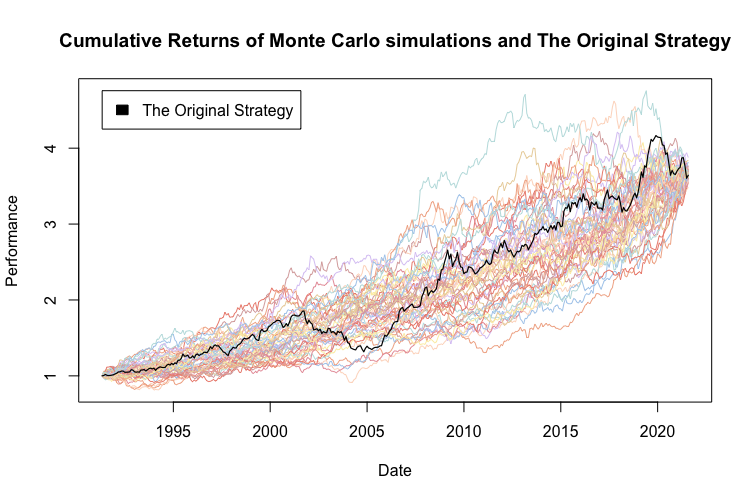
\includegraphics[width=\linewidth]{investment_simulation_process.png}
\caption{Investment Simulation Process for Monte Carlo Analysis}
\label{fig:simulation_process}
\end{figure}

\subsubsection{Expected Value and Risk Analysis}
The expected value and risk (standard deviation) of the simulated investment outcomes provide critical insights into the potential performance of different investment strategies. This analysis helps in identifying the strategies that offer the best balance between return and risk, tailored to the specific needs of first-time homebuyers.
